\section{Zielsetzung}
Ziel ist es für eine unbekannte Probe die aktiven Isotope und deren Aktivität zu ermitteln,
dafür ist es zuvor notwendig mit bekannten Elementen die Detektoreigenschaften
zu bestimmen.

\section{Theorie}
\subsection{Wechselwirkung von Strahlung mit Materie}
Wechselwirkt Strahlung mit Materie, so wird die Intensität der Strahlung durch das Material
abgeschwächt, diese Intensitätsabnahme kann allgemein über das Lambert-Beersche-Gesetz beschrieben werden:
\begin{equation}
  I(x)=I_0\cdot\exp(-\mu x).
  \label{eqn:lambert}
\end{equation}
Dabei bezeichnet $\mu$ den Extinktionskoeffizienten oder auch Abschwächungskoeffizient genannt, dieser
setzt sich aus Absorption und Streuung zusammen und lässt sich durch die Formel
\begin{equation}
  \mu=Zn\sigma
\end{equation}
beschreiben. Z bezeichnet die Ordnungszahl des Materials, n die Teilchenzahldichte und $\sigma$ den
Wirkungsquerschnitt der sich aus den verschiedenen Wechselwirkungen zusammensetzt.
\begin{figure}[H]
  \centering
  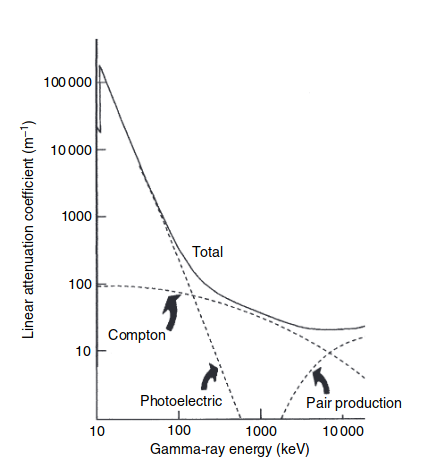
\includegraphics[height=8cm]{Extin.png}
  \caption{Der Extinkionskoeffizient in Abhängigkeit der Energie für verschiedene Prozesse. \cite{Gilmore2}}
  \label{fig:Extin}
\end{figure}

Wie in Abbildung \ref{fig:Extin} zu sehen ist, dominieren bei verschiedenen Energien
unterschiedliche Prozesse. Für geringe Energien dominiert der Photoeffekt, welcher mit
steigender Energie abnimmt, dadurch gewinnt der Comptoneffekt an Bedeutung. Für hohe
Energien dominiert die Paarerzeugung.
Da diese drei Prozesse für die Wechselwirkung von Gammaquanten mit Materie von großer Bedeutung sind
werden sie im Folgenden näher betrachtet.
\cite{Springer3}
\\
\\
\textbf{1. Photoeffekt}\\
Ein Gammaquant wird von einem kernnahen Hüllenelektron (bevorzugt aus der K-Schale) absorbiert,
wodurch das Hüllenelektron ausgelöst wird. Voraussetzung für diesen Effekt ist, dass das Gammaquant
mindestens die Bindungsenergie des Elektrons besitzt, überschüssige Energie wird als kinetische
Energie an das Elektron übertragen.
Das so entstandene "Loch" in der Elektronenhülle wird durch ein energiereicheres Hüllenelektron
gefüllt welches bei dem Übergang aus einer höheren Schale in eine niedrigere Schale
charakteristische Röntgenstrahlung emittiert.
Da sowohl die Röntgenstrahlung als auch das ausgelöste Elektron im Detektor verbleiben und
dort detektiert werden, verbleibt beim Photoeffekt die gesamte Gammaenergie im Detektor, weshalb
der Photopeak besonders wichtig für die Gammaspektroskopie ist.
Der differentielle Wirkungsquerschnitt der Energie lässt sich über die Formel
\begin{equation}
  \frac{d \sigma}{d E} = \bigg(-\frac{64}{7E^{9}}\bigg)^{1/2}\alpha^4 Z^5\sigma_{Th}
  \label{eqn:diffPhoto}
\end{equation}
beschreiben, wobei $\sigma_{Th}$ den Thomson-Wirkungsquerschnitt $\sigma_{Th} = \frac{8}{3}\pi r_{e}^2$
beschreibt mit $r_e$ als klassischen Elektronenradius.
(Thomson-Streuung: Streuung niederenergetischer Photonen an Elektronen) \cite{Springer3}
Der totale Wirkungsquerschnitt für den Photoeffekt ist von der Ordnungszahl des Materials
und der Photonenergie abhängig:
\begin{equation}
  \sigma_{\text{Photo}}\sim Z^5\cdot E_{\gamma}^{-7/2}.
  \label{eqn:WQphoto}
\end{equation}
\cite{Karlsruhe}
\\
\\

\textbf{2. Comptoneffekt}\\
Der Comptoneffekt beschreibt die Streuung von Photonen an äußeren Hüllenelektronen. Da
diese Streuung sehr stark winkelabhängig ist, kann von der gemessenen Elektronenenergie
nicht auf die Energie des Gammaquants geschlossen werden wodurch sich ein kontinuierliches
Spektrum, das Comptonkontinuum bildet. Dieses Spektrum bricht an der Comptonkante ab, hier
beträgt der Streuwinkel 180° und der Energieübertrag $E_{\text{max}}$ ist maximal, trotzdem gibt das
Gammaquant nicht seine gesamte Energie ab
\begin{equation}
  E_{max}=E_{\gamma}\cdot\frac{2\epsilon}{1+2\epsilon}\;\;<E_{\gamma}
  \label{eqn:kante}
\end{equation}
\cite{Springer3}.

Hier ist der Wirkungsquerschnitt über die Klein-Nishina-Formel gegeben, aus dieser ergibt sich der
differentielle Wirkungsquerschnitt:
\begin{equation}
  \frac{d\sigma}{dE}=\frac{3}{8}\sigma_{\text{Th}}\frac{1}{m_0 c^2 e^2}\bigg(2+\bigg(\frac{E}{h\nu-E} \bigg)^2 \bigg[\frac{1}{\epsilon^2}+
  \frac{h\nu-E}{h\nu}-\frac{2}{\epsilon}\bigg(\frac{h\nu-E}{h\nu}\bigg) \bigg]\bigg)
  \label{eqn:diffCompton}
\end{equation}
mit $\epsilon=\sfrac{E_{\gamma}}{m_e c^2}$.
Für den totalen Wirkungsquerschnitt gilt der Zusammenhang
\begin{equation}
  \sigma_{\text{Compton}}\sim \frac{Z}{E_{\gamma}}.
  \label{eqn:WPCompton}
\end{equation}
\\
\\
\textbf{3. Paarerzeugung}\\
Sind die Photonen energiereich genug können Elektron-Positron-Paare erzeugt werden, dafür müssen
die Photonen eine Mindestenergie von $E=2 m_0 c^2$ besitzen, also die doppelte
Ruheenergie des Elektrons.
Das so entstandene Positron annihiliert mit den im Detektor vorhandenen Elektronen und es
entstehen zwei Photonen. Wenn beide Photonen den Detektor verlassen wird dies als double-escape
bezeichnet, verlässt nur eins den Detektor entsteht der single-escape Peak.
Der differentielle Wirkungsquerschnitt für den Prozess der Paarerzeugung ist durch
\begin{equation}
  \frac{d\sigma}{dE}= \frac{28\alpha Z^2 r_{e}^2}{9E_{\gamma}}
  \label{eqn:diffPaar}
\end{equation}
gegeben, während der totale Wirkungsquerschnitt folgende Proportionalität besitzt:
\begin{equation}
  \sigma_{\text{Paar}}\sim Z^2\cdot\ln\Bigg(\frac{2E_{\gamma}}{m_e c^2}\Bigg).
  \label{eqn:WQPaar}
\end{equation}
\\

Eine Übersicht über die möglichen Wechselwirkungen von Gammaquanten mit Materie liefert
Abbildung \ref{fig:Effekt}.
\begin{figure}[H]
  \centering
  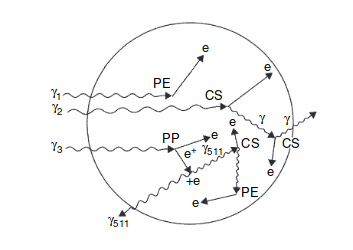
\includegraphics[height=5cm]{Effekte.png}
  \caption{Übersicht der Prozesse im Detektor. \cite{Gilmore2}}
  \label{fig:Effekt}
\end{figure}


\subsection{Grundlagen der Halbleiterinstrumente}
Halbleiter werden zwischen direkten und indirekten Halbleitern unterschieden, dies wird
in Abbildung \ref{fig:Band} dargestellt. Bei direkten Halbleitern
liegt das Maximum des Valenzbands genau unter dem Minimum des Leitungsbandes, somit ist ein direkter Bandübergang möglich.
Bei indirekten Halbleitern liegen Minima und Maxima nicht übereinander, für diesen indirekten Bandübergang ist
ein weiteres Phonon nötig.\\

\begin{figure}
  \centering
  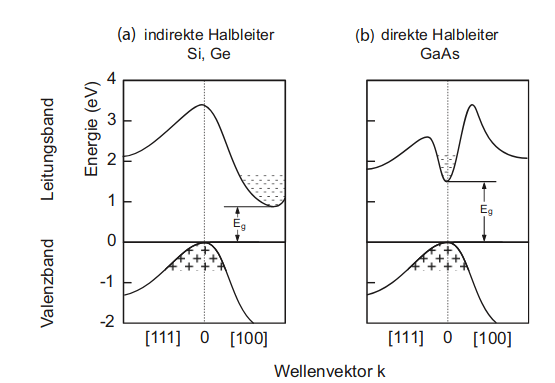
\includegraphics[height=6cm]{Band.png}
  \caption{Bandstruktur für direkte und indirekte Halbleiter.}
  \label{fig:Band}
  \cite{Springer3}
\end{figure}

Außerdem werden die Eigenschaften von Halbleitern durch ihre Dotierung beeinflusst. Germanium besitzt
beispielsweise 4 Valenzelektronen, wird nun ein Material mit fünf Valenzelektronen hinzugegeben bleibt nach
Eingehen der Bindungen ein freies Elektron übrig, somit dominieren die Elektronen als Ladungsträger und es handelt
sich um einen n-dotierten Halbleiter.
Wird stattdessen ein dreiwertiges Element verwendet bleibt ein Loch, somit stehen die Löcher als
positive Ladungsträger zur Verfügung und es handelt sich um einen p-dotierten Halbleiter.\\

\begin{figure}[H]
  \centering
  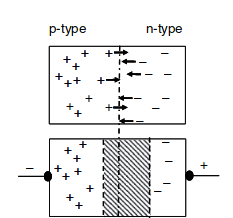
\includegraphics[height=6cm]{pn.png}
  \caption{Bildung einer Verarmungsschicht im pn-Übergang und Verbreiterung dieser durch
  anlegen einer äußeren Spannung.}
  \label{fig:pn}
  \cite{Gilmore2}
\end{figure}

Wie in Abbildung \ref{fig:pn} gezeigt entsteht ein pn-Übergang wenn p- und n-dotierte Halbleiter zusammengebracht werden,
Elektronen und Löcher vernichten sich in einem Teilbereich wodurch eine Verarmungszone entsteht.
Durch anlegen einer äußeren Spannung kann die Größe der Verarmungszone verändert werden. Für die
Verwendung als Detektor ist eine große Verarmungszone gewünscht, da dieser Bereich den
Detektorbereich bildet, also wird die Spannung in Sperrrichtung angelegt.


\subsection{Der Halbleiterdetektor}
Bei dem verwendeten Detektor handelt es sich um einen koaxialen Ge-Detektor wie in Abbildung
\ref{fig:Aufbau} zu sehen ist. Der gesamte Detektor befindet sich unter einer Aluminium
Schutzhaube und ist von außen mit Li-Atomen n-dotiert, wodurch die Oberfläche
gut leitend wird. Im Inneren befindet sich eine Bohrung, diese innere Oberfläche ist
mit Au-Atomen p-dotiert. (Die Dotierung ist hier etwas anders als oben beschrieben, da es sich um
Metall-Halbleiterkontakte handelt.) An diese dotierten Schichten wird die
äußere Spannung angelegt, die n-dotierte Schicht dient als Anschluss für den Pluspol.
Durch die p- und n-dotierten Bereiche bildet sich eine
Verarmungszone im Detektor die den Detektorbereich bildet. Somit müssen die Gammaquanten erst
die Al-Schicht und die Li-Schicht durchdringen um detektiert zu werden, dadurch kommt es zu einer
unteren Nachweisenergie der Gammaenergie, diese liegt bei 40 bis 50\;keV.
Dieser gesamte Aufbau, wie in Abbildung \ref{fig:Aufbau} gezeigt befindet sich in einem
Bleigehäuse welches von innen mit Kupferplatten ausgelegt ist. Das Bleigehäuse dient zur Abschirmung
äußerer Strahlung, während die Kupferplatten die aus dem Blei austretende Strahlung
abhalten sollen.

\begin{figure}
  \centering
  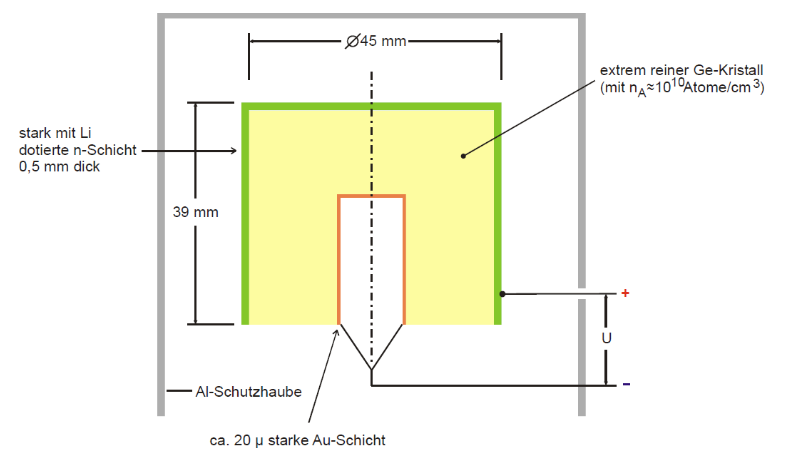
\includegraphics[height=7cm]{Aufbau.png}
  \caption{Schematischer Aufbau des Ge-Detektors. \cite{skript}}
  \label{fig:Aufbau}
\end{figure}

Dringt ein Gammaquant in die Verarmungszone ein wechselwirkt es mit der Materie und kann
z.B. ein Elektron auslösen welches mit anderen Elektronen stößt und ein Elektronen-Loch-Paar erzeugt.
Durch die angelegte Spannung wird das Paar räumlich getrennt wodurch eine Rekombination verhindert wird,
der dadurch entstehende Ladungsimpuls
wird verstärkt und bildet das Detektorsignal. Dieses ist proportional zu der einfallenden Photonenergie, da mit
einer höheren Energie auch mehr Elektronen-Loch-Paare erzeugt werden können.
Dringt das Gammaquant außerhalb der Verarmungszone in den Detektor ein rekombinieren die
Elektronen-Loch-Paare sofort, somit kann kein Signal gemessen werden.\\
Um Störsignale zu minimieren wird der Detektor mit Stickstoff auf 77\;K gekühlt, denn durch die
hohe externe Spannung kommt es zu thermischen Effekten wodurch sich noch Ladungsträger in der Verarmungszone
befinden und das Signal stören können.
\\
\\
\textbf{Eigenschaften eines Halbleiterdetektors}\\
Eine charakteristische Größe des Detektors ist das Auflösungsvermögen, dieses wird durch die
Halbwertsbreite $\Delta E_{1/2}$ der Impulshöhenverteilung beschrieben. Energien mit den Mittelwerten
$E_1$ und $E_2$ können noch voneinander unterschieden werden, wenn der Energieunterschied mindestens
$\Delta E_{1/2}$ beträgt.

Die Vollenergienachweiswahrscheinlichkeit eines Detektors gibt die Nachweiswahrscheinlichkeit eines Detektors
in Abhängigkeit der Energie an. Um sie zu bestimmen wird aus der aktuellen Aktivität der Probe der
theoretische Linieninhalt bestimmt, der Quotient aus gemessenem Linieninhalt und theoretischem
Linieninhalt gibt die Nachweiswahrscheinlichkeit des Detektors an.

\subsection{Das Spektrum eines monochromatischen Gammastrahlers}
Das Spektrum eines monochromatischen Gammastrahlers zeigt mehrere Besonderheiten auf, wie in Abbildung \ref{fig:Spektrum} zu
sehen. Wesentliche Bestandteile sind das Comptonkontinuum mit der Comptonkante, der Rückstreupeak
und der Photopeak. Der Photopeak entsteht dadurch, dass die Gammaquanten ihre gesamte Energie im Detektor deponieren
und wird daher auch Vollenergiepeak genannt. Er entsteht wenn die Gammaquanten im Detektor durch
Comptonstreuung genügend Energie verlieren bis der Photoeffekt eintreten kann und die restliche Energie
an den Detektor abgegeben wird. Auf diese Weise deponieren die Gammaquanten ihre gesamte Energie im
Detektor, so dass das Maximum des Photopeaks die Energie der Gammastrahlung angibt.\\
Das Comptonkontinuum entsteht durch Comptonstreuung der Gammaquanten, erfolgt die Streuung im
180° Winkel wobei der Energieübertrag maximal ist entsteht die Comptonkante. Da durch mehrfache
Comptonstreuung ein größerer Energieübertrag möglich ist als duch eine einmalige Streuung im 180° Winkel ist die
Componkante ausgeschmiert.\\
Da die Strahlung der Probe keine Vorzugsrichtung hat, wechselwirken einige Gammaquanten auch mit der
Abschirmung des Detektors und verlieren so Energie, werden sie dann so zurückgestreut, dass sie den
Detektor erreichen bilden sie den Rückstreupeak, dieser liegt bei
\begin{equation}
  E_{\text{Rück}}=E_{\gamma}\frac{1}{1+2\epsilon}
  \label{eqn:Rückstreu}
\end{equation}
Zwei weitere mögliche Peaks sind double- und single-escape Peak. Fällt ein Gammaquant in den Detektor und wechselwirkt über
Paarerzeugung entsteht ein Elektron und ein Positron, das Positron annihiliert mit den Elektronen der umgebenden Materie wobei
zwei Photonen erzeugt werden. Verlässt eins dieser Photonen den Detektor komm es zu single-escape Peak, verlassen beide
Photonen den Detektor entsteht der double-escape Peak.
\cite{Gilmore2}


\begin{figure}
  \centering
  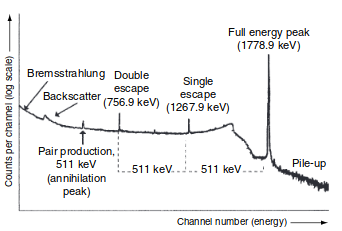
\includegraphics[height=7cm]{Spektrum.png}
  \caption{Gammaspektrum von $\ce{^{28}Al}$. Die Componkante ist hier nicht eingezeichnet, sie ist der Peak zwischen single escape und Photopeak,
  das Comptonkontinuum verläuft von der y-Achse bis zur Comptonkante.}\cite{Gilmore2}
  \label{fig:Spektrum}
\end{figure}
